\usetikzlibrary{decorations.pathmorphing}
\usetikzlibrary{arrows.meta}
\tikzset{snake it/.style={decorate, decoration=snake}}

%----------------------------------------
%Commands
%----------------------------------------
\newcommand{\textblue}[1]{ \color{blue}#1\color{black} }
\newcommand{\textred}[1]{ \color{red}#1\color{black} }
\newcommand{\textgreen}[1]{ \color{red}#1\color{black} }
%----------------------------------------
%Analysis
%----------------------------------------
\newcommand{\bsmumu}{B_{s}^{0}\rightarrow \mu^{+}\mu^{-}}
\newcommand{\bpjpsik}{B^{+}\rightarrow J/\psi+K^{+}}
\newcommand{\bsjpsiphi}{B_{s}^{0}\rightarrow J/\psi + \phi}

\newcommand{\bbmumux}{b\bar{b}\rightarrow\mu^+\mu^-+X}
\newcommand{\bbjpsix}{b\bar{b}\rightarrow J/\psi+X}
%----------------------------------------
%Useful to make diagrams
%----------------------------------------
\newcommand\tikzwidth{3}
\newcommand\tikzwidthwide{3}
\newcommand\tikzheight{0.25}
\newcommand\tikzdec{0.9}

\usetikzlibrary{shapes.geometric, arrows}
\tikzstyle{Round-rectangle-trans} = [rectangle, rounded corners, minimum width=\tikzwidth cm, minimum height=\tikzheight cm,text centered, text width=\tikzwidth cm, draw=white, fill=white!30]
\tikzstyle{Round-rectangle-white} = [rectangle, rounded corners, minimum width=\tikzwidth cm, minimum height=\tikzheight cm,text centered, text width=\tikzwidth cm, draw=black, fill=white!30]
\tikzstyle{Round-rectangle-blue} = [rectangle, rounded corners, minimum width=\tikzwidth cm, minimum height=\tikzheight cm,text centered, text width=\tikzwidth cm, draw=black, fill=blue!30]
\tikzstyle{Round-rectangle-green} = [rectangle, rounded corners, minimum width=\tikzwidth cm, minimum height=\tikzheight cm,text centered, text width=\tikzwidth cm, draw=black, fill=green!50]
\tikzstyle{Round-rectangle-red} = [rectangle, rounded corners, minimum width=\tikzwidth cm, minimum height=\tikzheight cm,text centered, text width=\tikzwidth cm, draw=black, fill=red!50]

\tikzstyle{Round-rectangle-trans-wide} = [rectangle, rounded corners, minimum width=\tikzwidthwide cm, minimum height=\tikzheight cm,text centered, text width=\tikzwidth cm, draw=white, fill=white!30]
\tikzstyle{Round-rectangle-white-wide} = [rectangle, rounded corners, minimum width=\tikzwidthwide cm, minimum height=\tikzheight cm,text centered, text width=\tikzwidth cm, draw=black, fill=white!30]
\tikzstyle{Round-rectangle-blue-wide} = [rectangle, rounded corners, minimum width=\tikzwidthwide cm, minimum height=\tikzheight cm,text centered, text width=\tikzwidth cm, draw=black, fill=blue!30]
\tikzstyle{Round-rectangle-green-wide} = [rectangle, rounded corners, minimum width=\tikzwidthwide cm, minimum height=\tikzheight cm,text centered, text width=\tikzwidth cm, draw=black, fill=green!50]
\tikzstyle{Round-rectangle-red-wide} = [rectangle, rounded corners, minimum width=\tikzwidthwide cm, minimum height=\tikzheight cm,text centered, text width=\tikzwidth cm, draw=black, fill=red!50]

\tikzstyle{rectangle-trans} = [rectangle, minimum width=\tikzwidth cm, minimum height=\tikzheight cm,text centered, text width=\tikzwidth cm, draw=white, fill=white!30]
\tikzstyle{rectangle-white} = [rectangle, minimum width=\tikzwidth cm, minimum height=\tikzheight cm,text centered, text width=\tikzwidth cm, draw=black, fill=white!30]
\tikzstyle{rectangle-blue} = [rectangle, minimum width=\tikzwidth cm, minimum height=\tikzheight cm,text centered, text width=\tikzwidth cm, draw=black, fill=blue!30]
\tikzstyle{rectangle-green} = [rectangle, minimum width=\tikzwidth cm, minimum height=\tikzheight cm,text centered, text width=\tikzwidth cm, draw=black, fill=green!50]
\tikzstyle{rectangle-red} = [rectangle, minimum width=\tikzwidth cm, minimum height=\tikzheight cm,text centered, text width=\tikzwidth cm, draw=black, fill=red!50]

\tikzstyle{rectangle-trans-wide} = [rectangle, minimum width=\tikzwidthwide cm, minimum height=\tikzheight cm,text centered, text width=\tikzwidth cm, draw=white, fill=white!30]
\tikzstyle{rectangle-white-wide} = [rectangle, minimum width=\tikzwidthwide cm, minimum height=\tikzheight cm,text centered, text width=\tikzwidth cm, draw=black, fill=white!30]
\tikzstyle{rectangle-blue-wide} = [rectangle, minimum width=\tikzwidthwide cm, minimum height=\tikzheight cm,text centered, text width=\tikzwidth cm, draw=black, fill=blue!30]
\tikzstyle{rectangle-green-wide} = [rectangle, minimum width=\tikzwidthwide cm, minimum height=\tikzheight cm,text centered, text width=\tikzwidth cm, draw=black, fill=green!50]
\tikzstyle{rectangle-red-wide} = [rectangle, minimum width=\tikzwidthwide cm, minimum height=\tikzheight cm,text centered, text width=\tikzwidth cm, draw=black, fill=red!50]

\tikzstyle{startstop} = [rectangle, rounded corners, minimum width=\tikzwidth cm, minimum height=\tikzheight cm,text centered, text width=\tikzwidth cm, draw=black, fill=red!30]
\tikzstyle{io} = [trapezium, trapezium left angle=70, trapezium right angle=110, minimum width=\tikzwidth cm, minimum height=\tikzheight cm, text centered, draw=black, fill=blue!30]
\tikzstyle{process} = [rectangle, minimum width=\tikzwidth cm, minimum height=\tikzheight cm, text centered, text width=\tikzwidth cm, draw=black, fill=orange!30]
\tikzstyle{decision} = [circle, minimum width=\tikzdec cm, minimum height=\tikzdec cm, text centered, text width=\tikzdec cm, draw=black, fill=green!30]
\tikzstyle{arrow} = [thick,->,>=stealth]
%----------------------------------------



\section{Background Modeling}
\label{sec:BackgroundModeling}

\subsection{Non-resonant Background}
\label{sub:sec:continuum}


The measurement of the rare decay of $B$ mesons into muon pairs
requires the rejection of a very large combinatorial background.
After the preliminary and additional selection, the amount of combinatorial
background is at the level of \yel[numbers t.b.u.]{$\approx$140~k events per 100~MeV} interval
in the muon pair invariant mass (this is shown in the context of the
normalisation study for the signal fit in Figure~\ref{fig:sbvars}).
This figure should be compared to $\approx$20 events/100~MeV expected
at the peak of the \Bs\ signal (section~\ref{sub:sec:bkg-normalisation-fit}).  

To have a statistically meaningful sample of this combinatorial background,
a very large number of events needs to be generated
(one of the largest MC production performed so far by ATLAS for a single analysis), 
thus specific procedures have been used in order to reduce the event generation
time, as discussed below.  
The MC sample was generated inclusively to provide a realistic composition of muons
from different sources, including non combinatorial sources of muon pairs. 
On the other hand, because of uncertainties in cross sections and branching ratios, 
as well as for those related to the generation procedures, 
%(repeated hadronisation and repeated decays)
no attempt is made to use the MC to draw quantitative conclusions
on the amount in which each type of background is present in real data.
For that purpose, events collected in the sidebands are used.
As shown in section~\ref{sub:sec:bkg-normalisation-fit}, after the background
reduction developed on MC is applied, the remaining background in real data is
sufficiently low and separated in its different components to be used for an
effective interpolation in the signal region. 

In order to optimise the production speed, {\em repeated hadronisation} and {\em repeated decay}
procedures were used for the inclusive MC, in order to reduce the typical generation time
from a several minutes per event to only about 40 seconds. 

Repeated hadronisation, performed in \Pythia, was applied with 10 repetitions. 
This is technically implemented by means of PythiaB
package~\cite{PythiaB} and had already been widely tested and used for various MC
production in $B$ physics. This procedure scarcely affects the characteristics of
the generated samples. 

The next step, decays of the unstable particles, has been done differently with respect to Run 1,
since the procedure employed back then effectively enhanced the acceptance at lower \pT, which
required a correction. Currently, each hadronised event is cloned fixed number of times (200) by \Pythia~and each cloned event
decays independently. In the next step a generator level filtering (e.g. cuts on muons transverse momenta) is applied, 
and all cloned events which pass it are stored in the resulting sample. 
This approach allows events with identical b hadron kinematics if more than one of those 200 
clones produce a muon pair, which passes the filter. 
However, this approach does not introduce the kinematic bias we had in Run 1. With
\Pythia (unlike \textsc{EvtGen} used in Run 1) we have less up-to-date decay tables 
and no angular decay models. However the last 
effect we found to be negligible for the decays we require - with two muons in the final state.
The residual descrepancies in kinematic of B-candidates and multiplicity of tracks in the vicinity
of reconsructed di-muon vertices are corrected on data.

If only standard cuts are applied to the
muons and loose cuts are applied to the muon pair, the MC sample is dominated
by opposite side combinatorial background (about \yel[numbers t.b.u.]{20~M events in the mass interval
4.8-5.9~GeV, with 50~k} events of different nature). When a multivariate selection
aiming at the rejection of combinatorial background is applied  (as discussed
in Sec~\ref{sec:contBDT}), the relevance of the additional contribution becomes
more evident (e.g., for a selection aiming at \yel[numbers t.b.u.]{60~\%  (20~\%) efficiency} for the signal
\Bsmumu, opposite side events account for about \yel[numbers t.b.u.]{95 \% (40 \%)} of the muon pairs
in the mass interval 4.8--5.9 GeV). The additional events are mainly due to
same-side combinatorial  background from $B$ meson decays, and also to exclusive
decays such as $\Bc^+ \to \Jpsi \, \mu^+ \nu$, $B \to K \, \mu^+\mu^- (\gamma)$,
$\Bs \to \mu^+ \mu^-(\gamma)$  (\yel[numbers t.b.u.]{XXX} signal events are present in the four-corner
MC sample).


Because of the uncertainties discussed above, information extracted from the relative
normalisation of the different types of backgrounds and of the signal events present
in the inclusive sample are not used in any part of the analysis.
On the other hand, the samples of data obtained from MC have shown
remarkable consistency with real data collected in the side-bands of the
signal region, in their dependence on the di-muon invariant mass and on
the BDT classifier.
It is also remarkable that the simulation shows that exclusive
semileptonic decays $\Bz \to \pi\mu\nu$, $\Bs \to K\mu\nu$, with the hadron being
misidentified as muon, provide a background of negligible size
compared to same-side cascade events, or \Bc\ background. 


\subsection{Background Classification}
\label{sub:sec:bkgclass}
\graphicspath{ {figures/InternalNote_BackgroundModeling/} }

The three processes of interest are $\bsmumu$, $\bpjpsik$ and $\bsjpsiphi$. In order to estimate the different
background contributions to each of them, the MC in table \ref{table:inclusive_mc} is used.

\begin{table}[h!]
    \centering
    \begin{tabular}{|l | c | r | l|} 
	\hline
	Process & DSID & Events & Generator\\ [0.5ex] 
	\hline
	\hline
	$\bbmumux$ & 300307 & 600M & PYTHIA + PHOTOS\\ 
	$\bbjpsix$ & 300203 & 10M & PYTHIA\\ [1ex] 
	\hline
    \end{tabular}
    \caption{Inclusive background samples used to find background contributions.}
    \label{table:inclusive_mc}
\end{table}

The same reconstruction algorithms that would be applied to the three exclusive MC samples
are applied to the inclusive samples. From this, containers with candidates misidentified as
$B_{s}^{0}$ and $B^{+}$ are created. The reconstructed objects, both muons and tracks can be 
matched to the corresponding truth objects. In this way, one can create a string representing the
decay process responsible for the reconstructed $B$ candidate. Figure \ref{fig:reco_truth_assoc_comb}
shows this, in this case, given that the upper most truth $B$ candidate does not exist (there are two,
each associated to a $b$ quark), this reconstructed $B_{s}^{0}$ would be combinatorial background.

\begin{figure}[ht]
    \centering
    \subfloat[Combinatorial background]
    {
	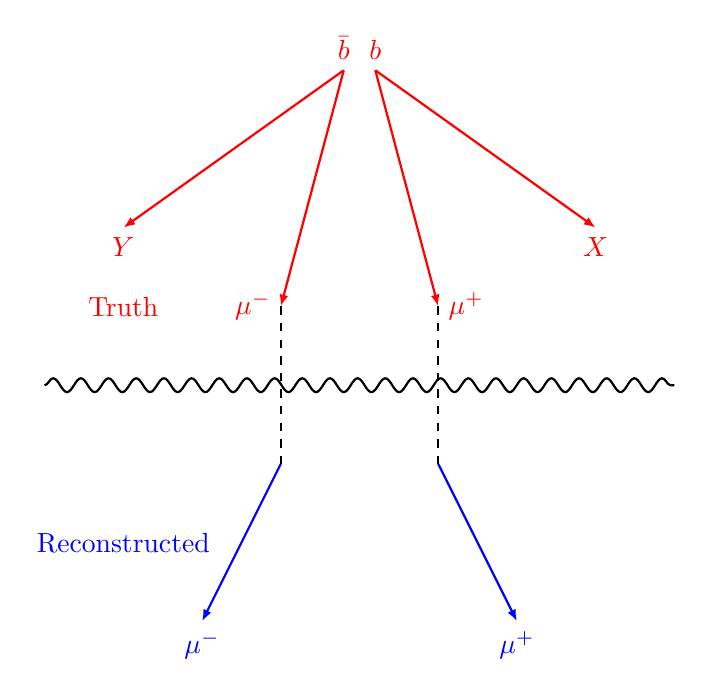
\begin{tikzpicture}[thick, scale = 1]
	    \draw[red,-{Latex[length=1.5mm]}](0.2,4) node[above]{$b$} (0.2,4)--(1,1) node[right]{$\mu^+$};
	    \draw[red,-{Latex[length=1.5mm]}](-0.2,4) node[above]{$\bar{b}$} (-0.2,4)--(-1,1) node[left]{$\mu^-$};

	    \draw[red,-{Latex[length=1.5mm]}] (0.2,4)--(3,2) node[below]{$X$};
	    \draw[red,-{Latex[length=1.5mm]}] (-0.2,4)--(-3,2) node[below]{$Y$};

	    \path [draw=black,snake it] (-4,0) -- (4,0);
	    \draw[dashed] (1,1)--(1,-1);
	    \draw[dashed] (-1,1)--(-1,-1);


	    \draw[blue,-{Latex[length=1.5mm]}] (1,-1)--(2,-3) node[below]{$\mu^+$};
	    \draw[blue,-{Latex[length=1.5mm]}] (-1,-1)--(-2,-3) node[below]{$\mu^-$};

	    \draw(-3,-2)node[fill=white, text=blue]{Reconstructed};
	    \draw(-3,+1)node[fill=white, text=red]{Truth};
	\end{tikzpicture}
	\label{fig:reco_truth_assoc_comb}
    }
    \subfloat[Partially reconstructed decay]
    {
	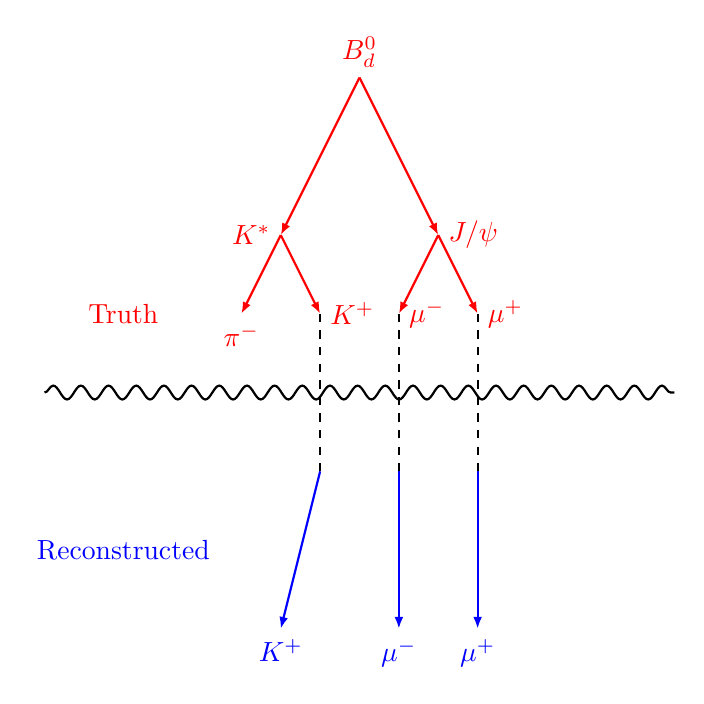
\begin{tikzpicture}[thick, scale = 1]
	    \draw[red,-{Latex[length=1.5mm]}](0,4)                          (0,4)--(-1,2) node[left]{$K^*$};
	    \draw[red,-{Latex[length=1.5mm]}] (-1,2)--(-0.5,1) node[right]{$K^+$};
	    \draw[red,-{Latex[length=1.5mm]}] (-1,2)--(-1.5,1) node[below]{$\pi^-$};

	    \draw[red,-{Latex[length=1.5mm]}](0,4) node[above]{$B_{d}^{0}$} (0,4)--(1,2) node[right]{$J/\psi$};
	    \draw[red,-{Latex[length=1.5mm]}] (1,2)--(1.5,1) node[right]{$\mu^+$};
	    \draw[red,-{Latex[length=1.5mm]}] (1,2)--(0.5,1) node[right]{$\mu^-$};

	    \path [draw=black,snake it] (-4,0) -- (4,0);

	    \draw[dashed] (1.5,1)--(1.5,-1);
	    \draw[dashed] (0.5,1)--(0.5,-1);
	    \draw[dashed] (-0.5,1)--(-0.5,-1);


	    \draw[blue,-{Latex[length=1.5mm]}] (1.5,-1)--(1.5,-3) node[below]{$\mu^+$};
	    \draw[blue,-{Latex[length=1.5mm]}] (0.5,-1)--(0.5,-3) node[below]{$\mu^-$};

	    \draw[blue,-{Latex[length=1.5mm]}] (-0.5,-1)--(-1,-3) node[below]{$K^+$};


	    \draw(-3,-2)node[fill=white, text=blue]{Reconstructed};
	    \draw(-3,+1)node[fill=white, text=red]{Truth};
	\end{tikzpicture}
	\label{fig:reco_truth_assoc_partial}
    }
    \caption{Both diagrams represent a reconstructed $B_{s}^0$ or $B^+$, which in reality are
    combinatorial background or a partially reconstructed decay.}
    \label{fig:reco_truth_assoc}
\end{figure}

On the other hand, figure \ref{fig:reco_truth_assoc_partial} shows a reconstructed $B^+$ candidate
originating from a partially reconstructed decay. In this case the decay string would be \textit{B0[K*0[pi-:K+]Jpsi[mu+:mu-]]}.\\

\subsubsection{Truth Matching}
Figures \ref{fig:reco_truth_assoc} show, as a dashed black line, the truth and reconstructed objects matching.
In order to match them one requires $\Delta R < 0.05$. Preliminary studies have shown that the optimal value for this
cone is $0.01$; but a larger radius should prevent us from loosing any truth candidate. In order to prevent truth objects that
are not associated with the reconstructed object, from entering the cone, we require:

\begin{equation}
    \left|1-\frac{p_T^{truth}}{p_T^{reco}}\right|<0.15
\end{equation}

Also, reconstructed muons are required to be matched to muons with the same charge. The kaons are required to be
matched with truth light hadrons, either mesons or baryons.

\subsubsection{Cumulative Decay Probability Distribution}
A natural question now would be, how many different events in the inclusive background survive the 
candidate selection and get reconstructed? Figure \ref{fig:bbjpsix_cutflow} shows the number of events and candidates
at each stage of the analysis, from the xAOD level until the ntuples.

\begin{figure}
    \centering
    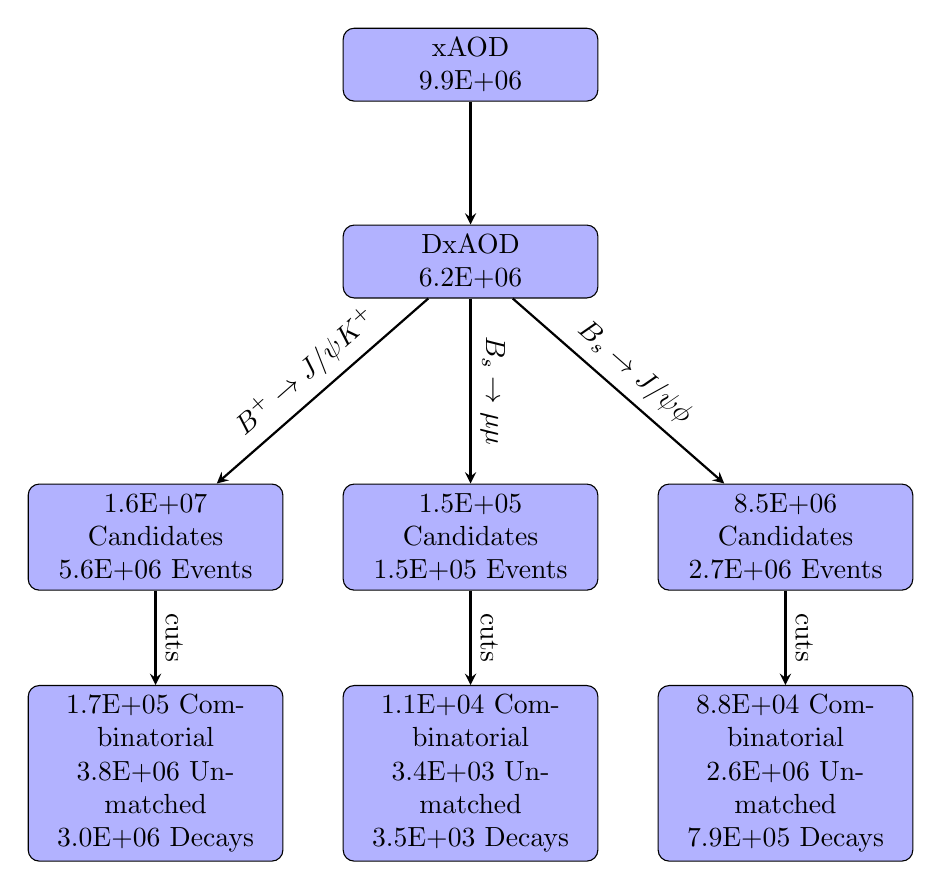
\begin{tikzpicture}[node distance=3cm]
	\node (xAOD)  [Round-rectangle-blue, xshift=-3cm] {xAOD\\ 9.9E+06};

	\node (DxAOD) [Round-rectangle-blue, yshift=0.5cm, below of=xAOD] {DxAOD\\ 6.2E+06};
	\draw [arrow, draw=black] (xAOD) --node[] {} (DxAOD);

	\node (NTP_B2) [Round-rectangle-blue, xshift=-4cm, yshift=-0.5cm, below of=DxAOD] {1.6E+07 Candidates\\5.6E+06 Events};
	\node (TREE_B2) [Round-rectangle-blue, yshift=0cm, below of=NTP_B2] {1.7E+05 Combinatorial\\3.8E+06 Unmatched\\3.0E+06 Decays};
	\draw [arrow, draw=black] (NTP_B2) --node[text centered, sloped, above] {cuts} (TREE_B2);

	\node (NTP_B1) [Round-rectangle-blue, xshift=0cm, yshift=-0.5cm, below of=DxAOD] {1.5E+05 Candidates\\1.5E+05 Events};
	\node (TREE_B1) [Round-rectangle-blue, yshift=0cm, below of=NTP_B1] {1.1E+04 Combinatorial\\3.4E+03 Unmatched\\3.5E+03 Decays};
	\draw [arrow, draw=black] (NTP_B1) --node[text centered, sloped, above] {cuts} (TREE_B1);

	\node (NTP_B3) [Round-rectangle-blue, xshift=+4cm, yshift=-0.5cm, below of=DxAOD] {8.5E+06 Candidates\\2.7E+06 Events};
	\node (TREE_B3) [Round-rectangle-blue, yshift=0cm, below of=NTP_B3] {8.8E+04 Combinatorial\\2.6E+06 Unmatched\\7.9E+05 Decays};
	\draw [arrow, draw=black] (NTP_B3) --node[text centered, sloped, above] {cuts} (TREE_B3);

	\draw [arrow, draw=black] (DxAOD) --node[text centered, sloped, above] {$B_{s}\rightarrow\mu\mu$} (NTP_B1);
	\draw [arrow, draw=black] (DxAOD) --node[text centered, sloped, above] {$B^{+}\rightarrow J/\psi K^{+}$} (NTP_B2);
	\draw [arrow, draw=black] (DxAOD) --node[text centered, sloped, above] {$B_{s}\rightarrow J/\psi \phi$} (NTP_B3);
    \end{tikzpicture}
    \caption{Cutflow corresponding to $\bbjpsix$ sample.}
    \label{fig:bbjpsix_cutflow}
\end{figure}

The cuts used in the last level are:

\begin{itemize}
    \item \textbf{Muons:} Combined muons that pass MCP requirements and $|\eta|<2.5$, $p_{T}>4GeV$.
    \item \textbf{Kaons:} Must pass loose requirements and $|\eta|<2.5$, $p_{T}>1GeV$.
    \item \textbf{Candidates:} $|\eta|<2.5$, $p_{T}>8GeV$, $\chi^{2}<6$.
\end{itemize}

Another thing that we might want to know is the number of decays present in the samples. Figure 
\ref{fig:decay_multiplicity} shows the cumulative distribution of decays vs the decay index, where the most
common decays are put first. From this we can conclude that, as expected, the $\bbmumux$ sample
contains very few $\bsmumu$ candidates and mostly $\bpjpsik$ and $\bsjpsiphi$ candidates.
Two mass windows were used, the wide window contains much more decays than the narrow one.
This is because in the low end of the mass spectrum, partially reconstructed decays, like the one
in \ref{fig:reco_truth_assoc_partial}, accumulate. The narrow mass window removes all of them.
Another thing that the plot tells us is that there are many more background processes associated
to the $\bsjpsiphi$ candidates than to the $\bpjpsik$ candidates.

\begin{figure}[ht]
    \centering
    \subfloat[\scriptsize $B_{s}\rightarrow\mu\mu$.]
    {
	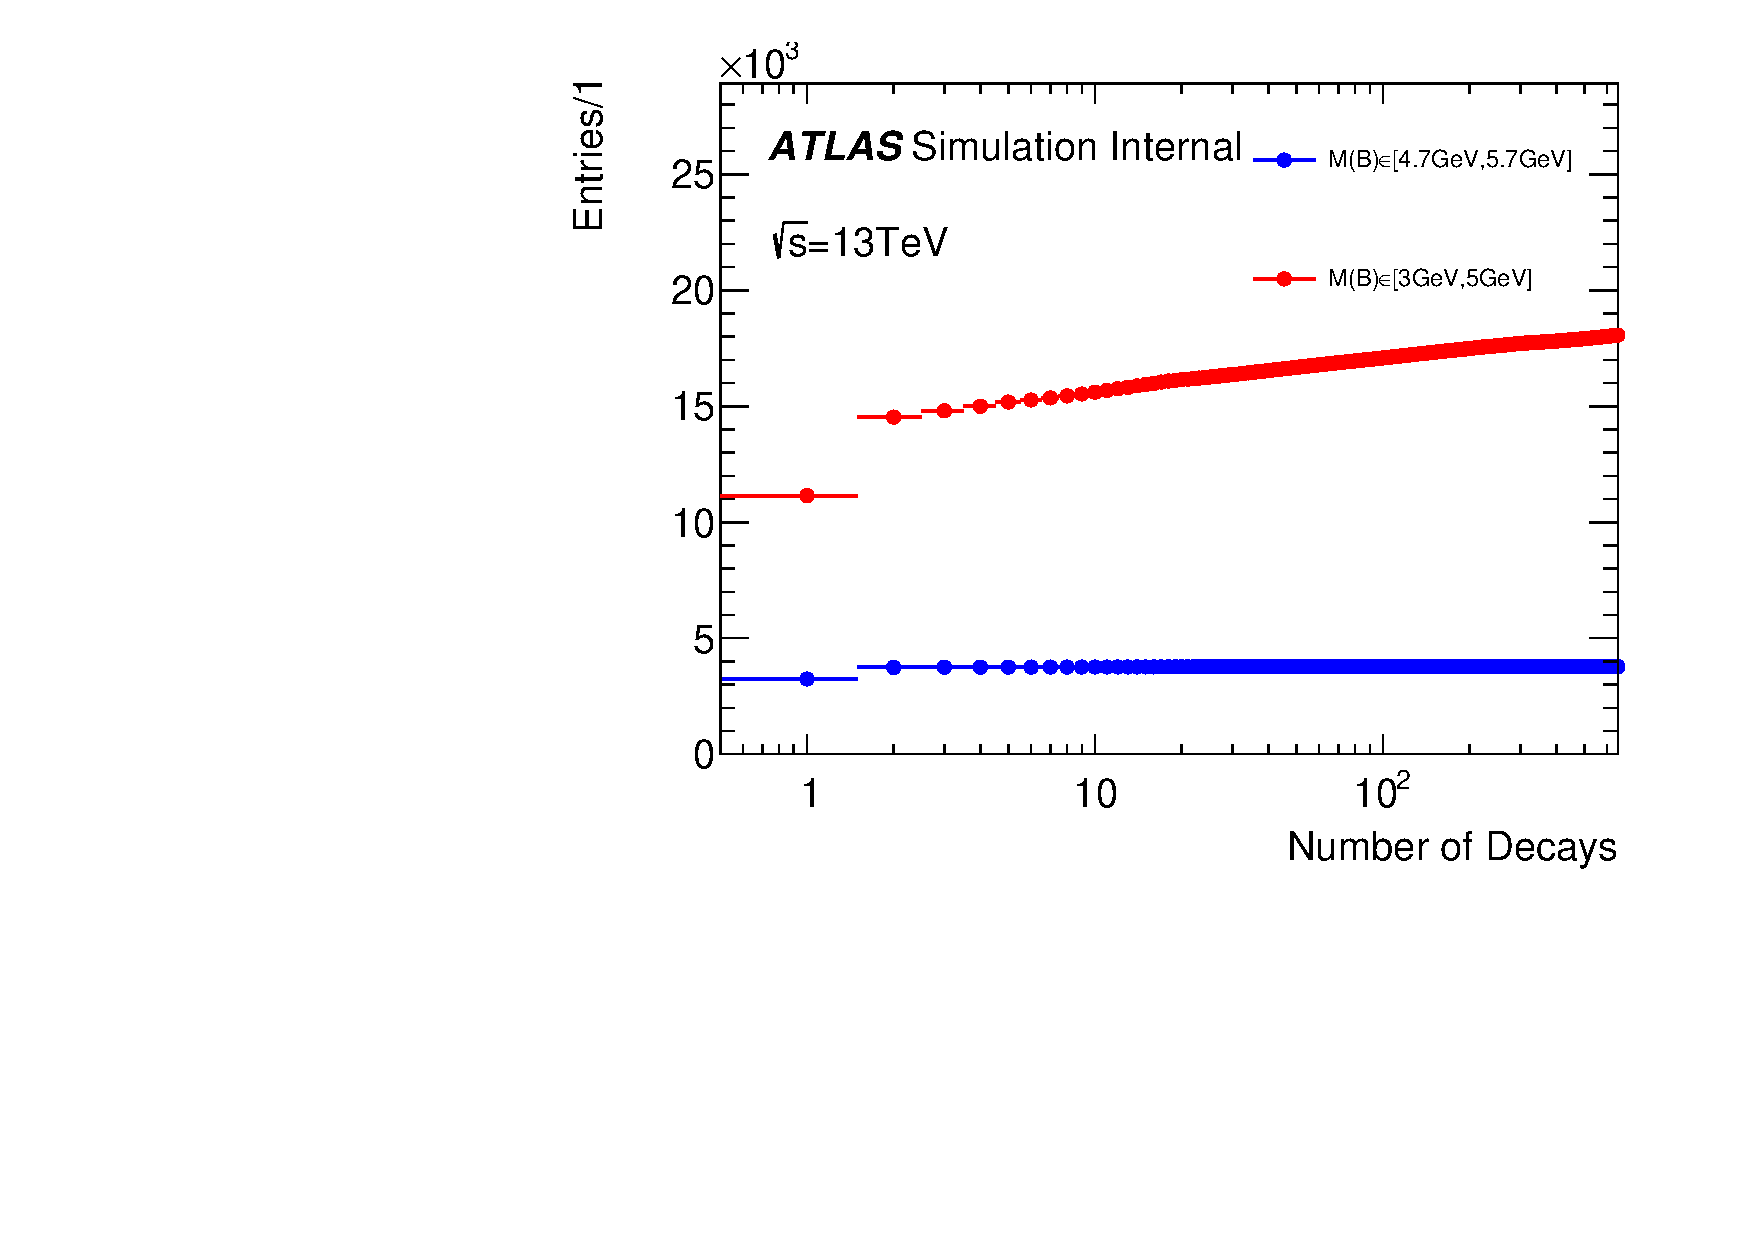
\includegraphics[width=0.45\textwidth]{bsmumu_decay_dist/cumul_entries}
    }
    \subfloat[\scriptsize $B^{+}\rightarrow J/\psi K^{+}$]
    {
	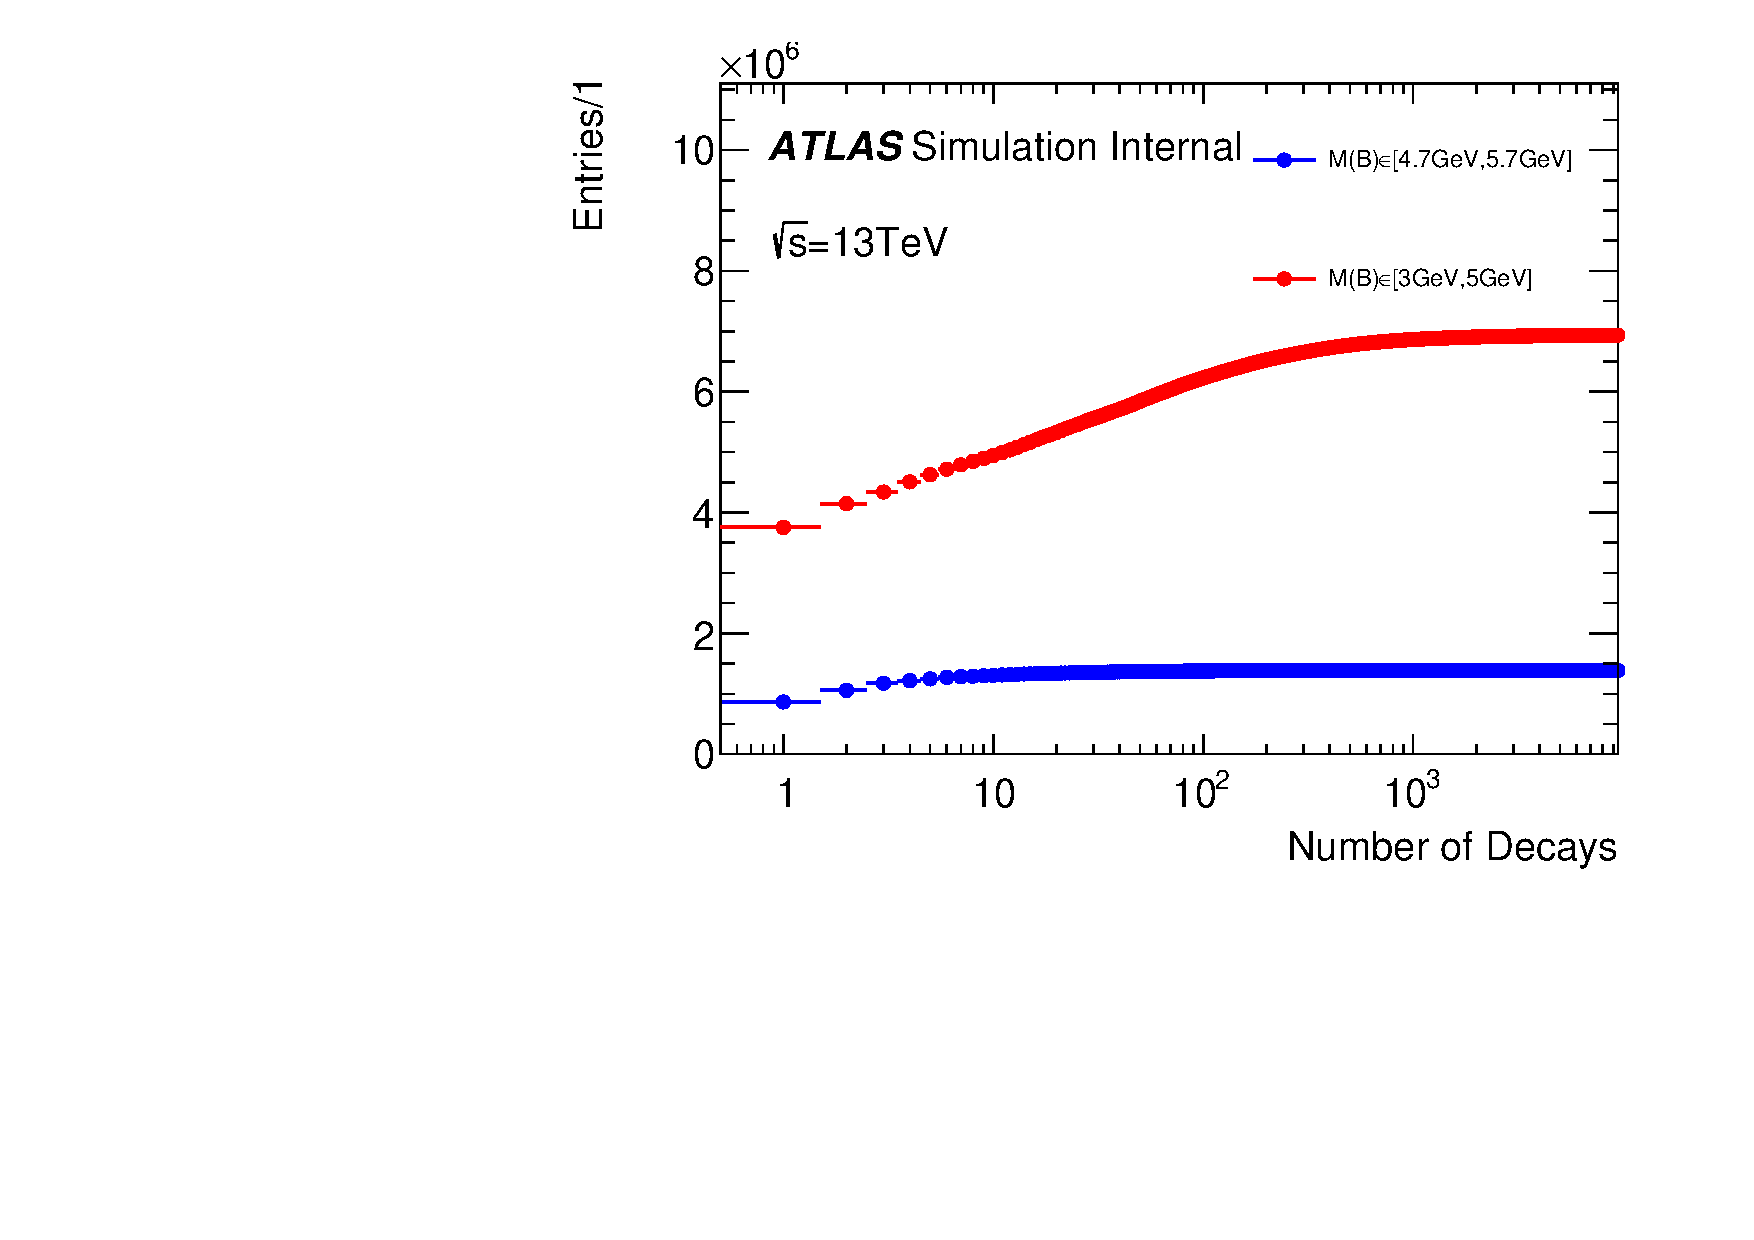
\includegraphics[width=0.45\textwidth]{bplus_decay_dist/cumul_entries}
    }

    \subfloat[\scriptsize $B_{s}\rightarrow J/\psi \phi$]
    {
	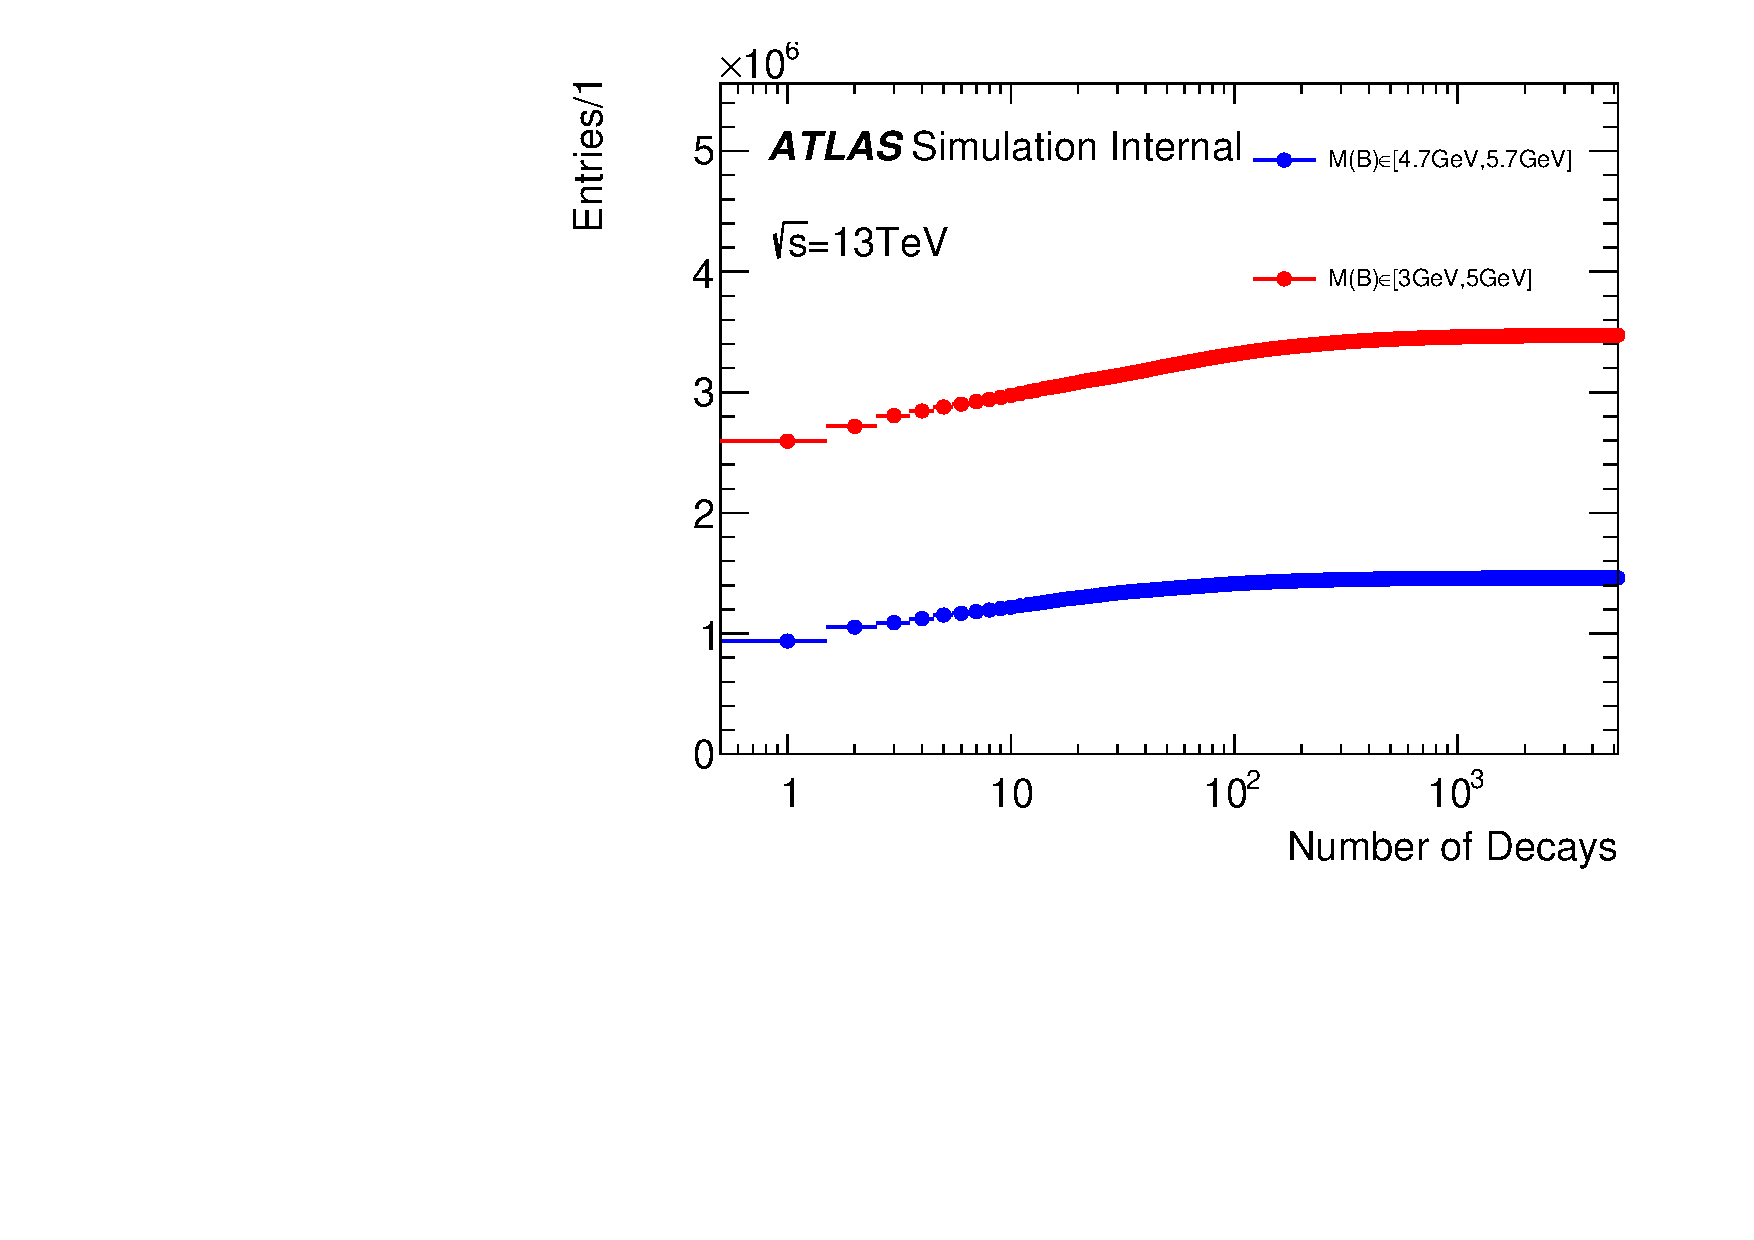
\includegraphics[width=0.45\textwidth]{bsjpsiphi_decay_dist/cumul_entries}
    }
    \caption{\scriptsize Both figures above show the cumulative number of events per decay. The first bin
	has all the events for decay number 1. The next bin, those plus decay 2, etc. The decays are ordered
    in decreasing order of events.}
    \label{fig:decay_multiplicity}
\end{figure}

Table \ref{tab:bpjpsik_decays} shows the main sources of background for $\bpjpsik$.
Table \ref{tab:bsjpsiphi_decays} shows the same for $\bsjpsiphi$. In these tables
\textit{unmatched} refers to decays in which the matching could not be made. This
happens because one of the hadron tracks, identified as the $K^+$, corresponds to
a particle that was removed from the samples during the derivation. In order to 
slim the truth particles container, particles that do not come from a $B$ decay
are removed. In practice this means that unmatched candidates can be classified
as combinatorial background. This can be seen in figure \ref{fig:unmatched_combinatorial}.

\begin{table}
    \centering
    \begin{tabular}{| l | r |}
	\hline
	Process                                           &     Candidates\\
	\hline
	unmatched                                         &         864837\\
	B+[K+:Jpsi[mu+:mu-]]                              &         192462\\
	B0[K*0[pi-:K+]Jpsi[mu+:mu-]]                      &         117439\\
	combinatorial                                              &          41869\\
	B+[K*+[pi0[gamma:gamma]K+]Jpsi[mu+:mu-]]          &          30063\\
	B+[K+:chi\_1c[gamma:Jpsi[mu+:mu-]]]                &         26241\\
	B+[K+:psi'[pi-:pi+:Jpsi[mu+:mu-]]]                &           9477\\
	B0[K*0[pi-:pi-:gamma:K+:K+]Jpsi[mu+:mu-]]         &           8545\\
	B0[pi-:K+:Jpsi[mu+:mu-]]                          &           7886\\
	B0[K*\_20[pi-:K+]Jpsi[mu+:mu-]]                    &          7435\\
	B+[pi+:Jpsi[mu+:mu-]]                             &           5956\\
	B+[K*+[pi+:K0[K\_L0]]Jpsi[mu+:mu-]]                &          5198\\
	B+[K*+[pi+:K0[K\_S0]]Jpsi[mu+:mu-]]                &          5087\\
	B+[K+:psi'[pi0[gamma:gamma]pi0[gamma:gamma]Jpsi[mu+:mu-]]]&   4811\\
	B+[rho+[pi0[gamma:gamma]pi+]Jpsi[mu+:mu-]]        &           3022\\
	\hline
    \end{tabular}
    \caption{Processes most commonly misidentified as $\bpjpsik$.}
    \label{tab:bpjpsik_decays}
\end{table}

\begin{table}
    \centering
    \begin{tabular}{| l | r |}
	\hline
	Process                                           &     Candidates\\
	\hline
	unmatched                                         &         759877\\
	B0[K*0[pi-:K+]Jpsi[mu+:mu-]]                      &         147001\\
	combinatorial                                              &          49979\\
	B0[Jpsi[mu+:mu-]K\_10[rho-[pi-:pi0[gamma:gamma]]K+]]&          43372\\
	B+[Jpsi[mu+:mu-]K\_1+[rho0[pi-:pi+]K+]]            &          33521\\
	B0[pi-:K+:Jpsi[mu+:mu-]]                          &          17924\\
	B0[K*0[pi-:K+]psi'[pi-:pi+:Jpsi[mu+:mu-]]]        &          16922\\
	B+[Jpsi[mu+:mu-]K\_1+[pi+:K*0[pi-:K+]]]            &          16325\\
	B0[pi-:K+:psi'[pi-:pi+:Jpsi[mu+:mu-]]]            &          14931\\
	B0[K*\_20[pi-:K+]Jpsi[mu+:mu-]]                    &          14856\\
	B+[K+:psi'[pi-:pi+:Jpsi[mu+:mu-]]]                &          13086\\
	B+[Jpsi[mu+:mu-]K\_1+[omega[pi-:pi0[gamma:gamma]pi+]K+]]&          12826\\
	B0[pi-:K+:chi\_1c[gamma:Jpsi[mu+:mu-]]]            &          12027\\
	B\_s0[phi[K-:K+]Jpsi[mu+:mu-]]                     &          11752\\
	B0[K*0[pi-:pi-:gamma:K+:K+]Jpsi[mu+:mu-]]         &          11022\\
	\hline
    \end{tabular}
    \caption{Processes most commonly misidentified as $\bsjpsiphi$.}
\end{table}

\begin{figure}[ht]
    \centering
    \subfloat[Combinatorial]
    {
	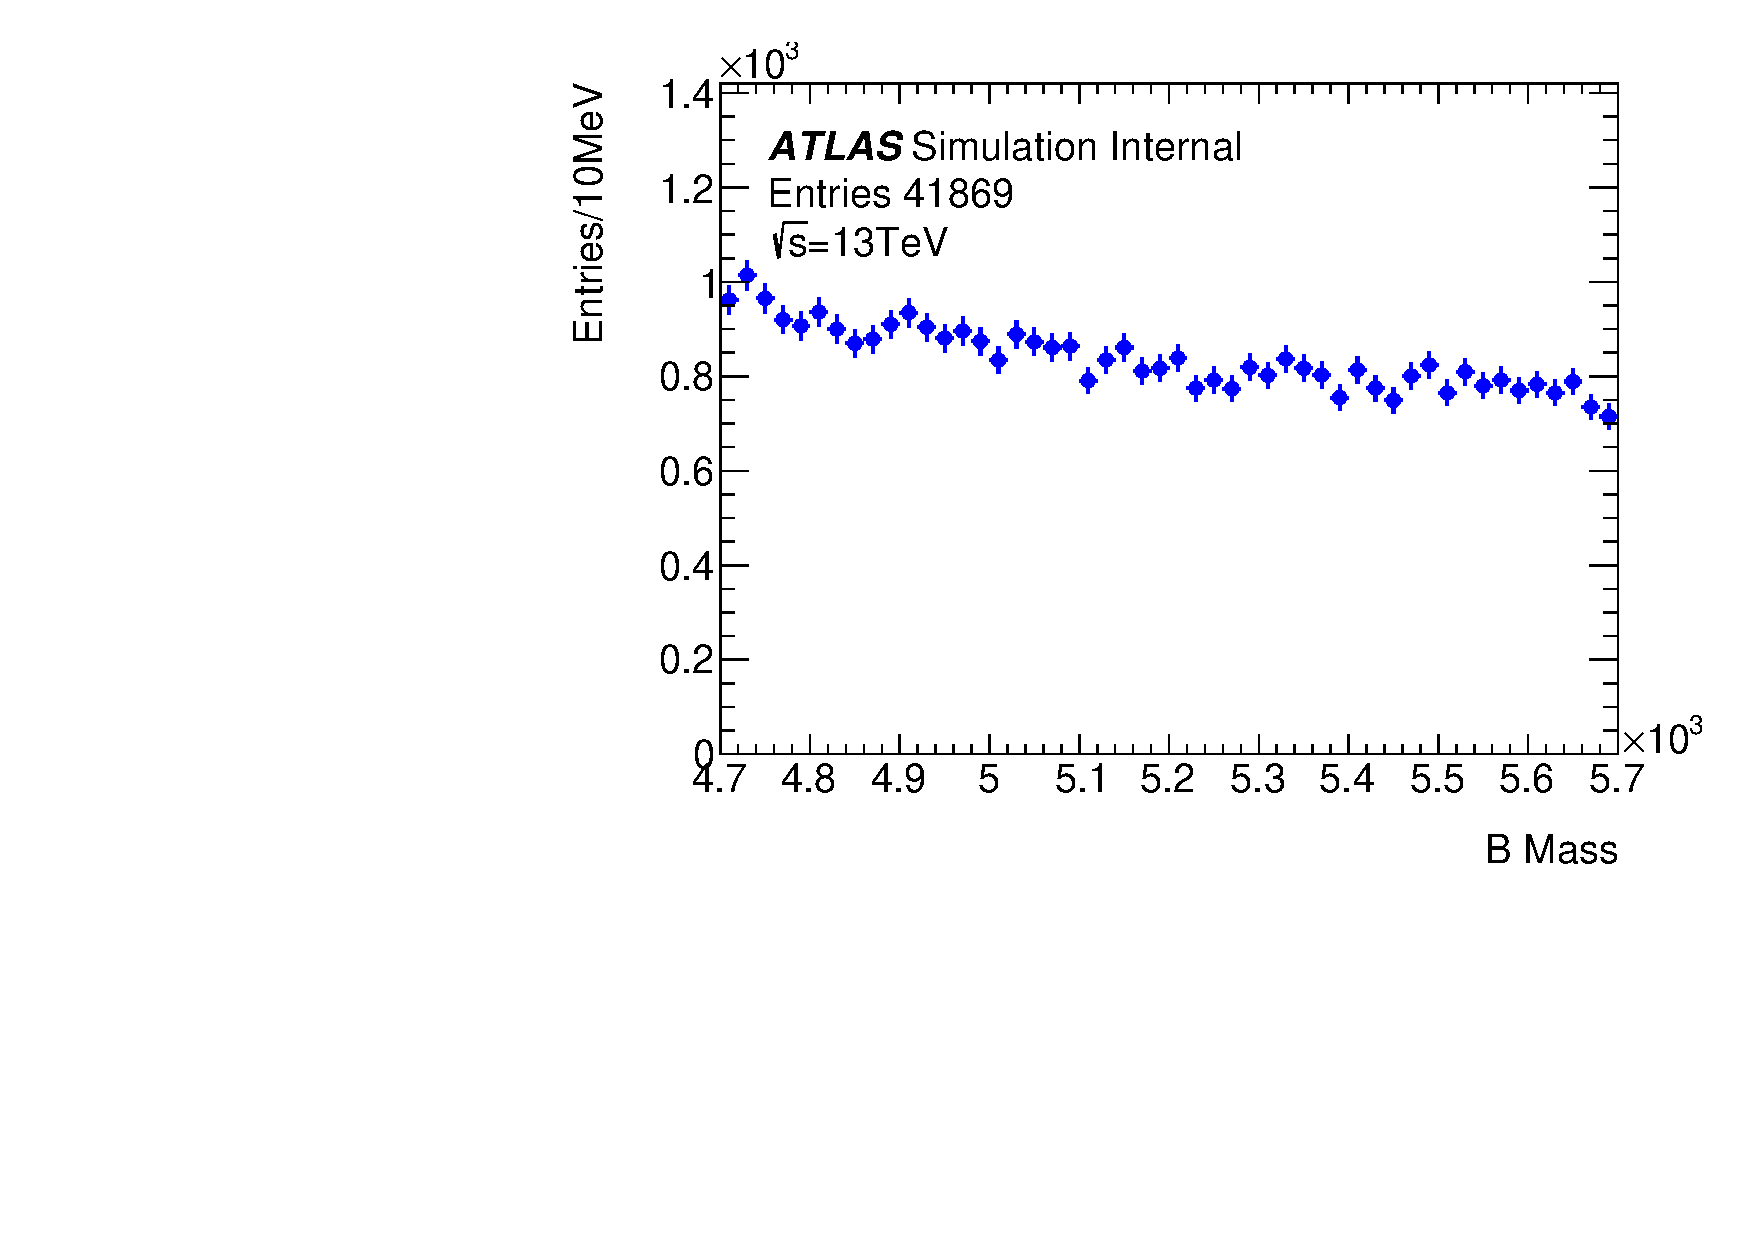
\includegraphics[width=0.45\textwidth]{bplus_components/narrow__41869__comb.pdf}
    }
    \subfloat[Unmatched]
    {
	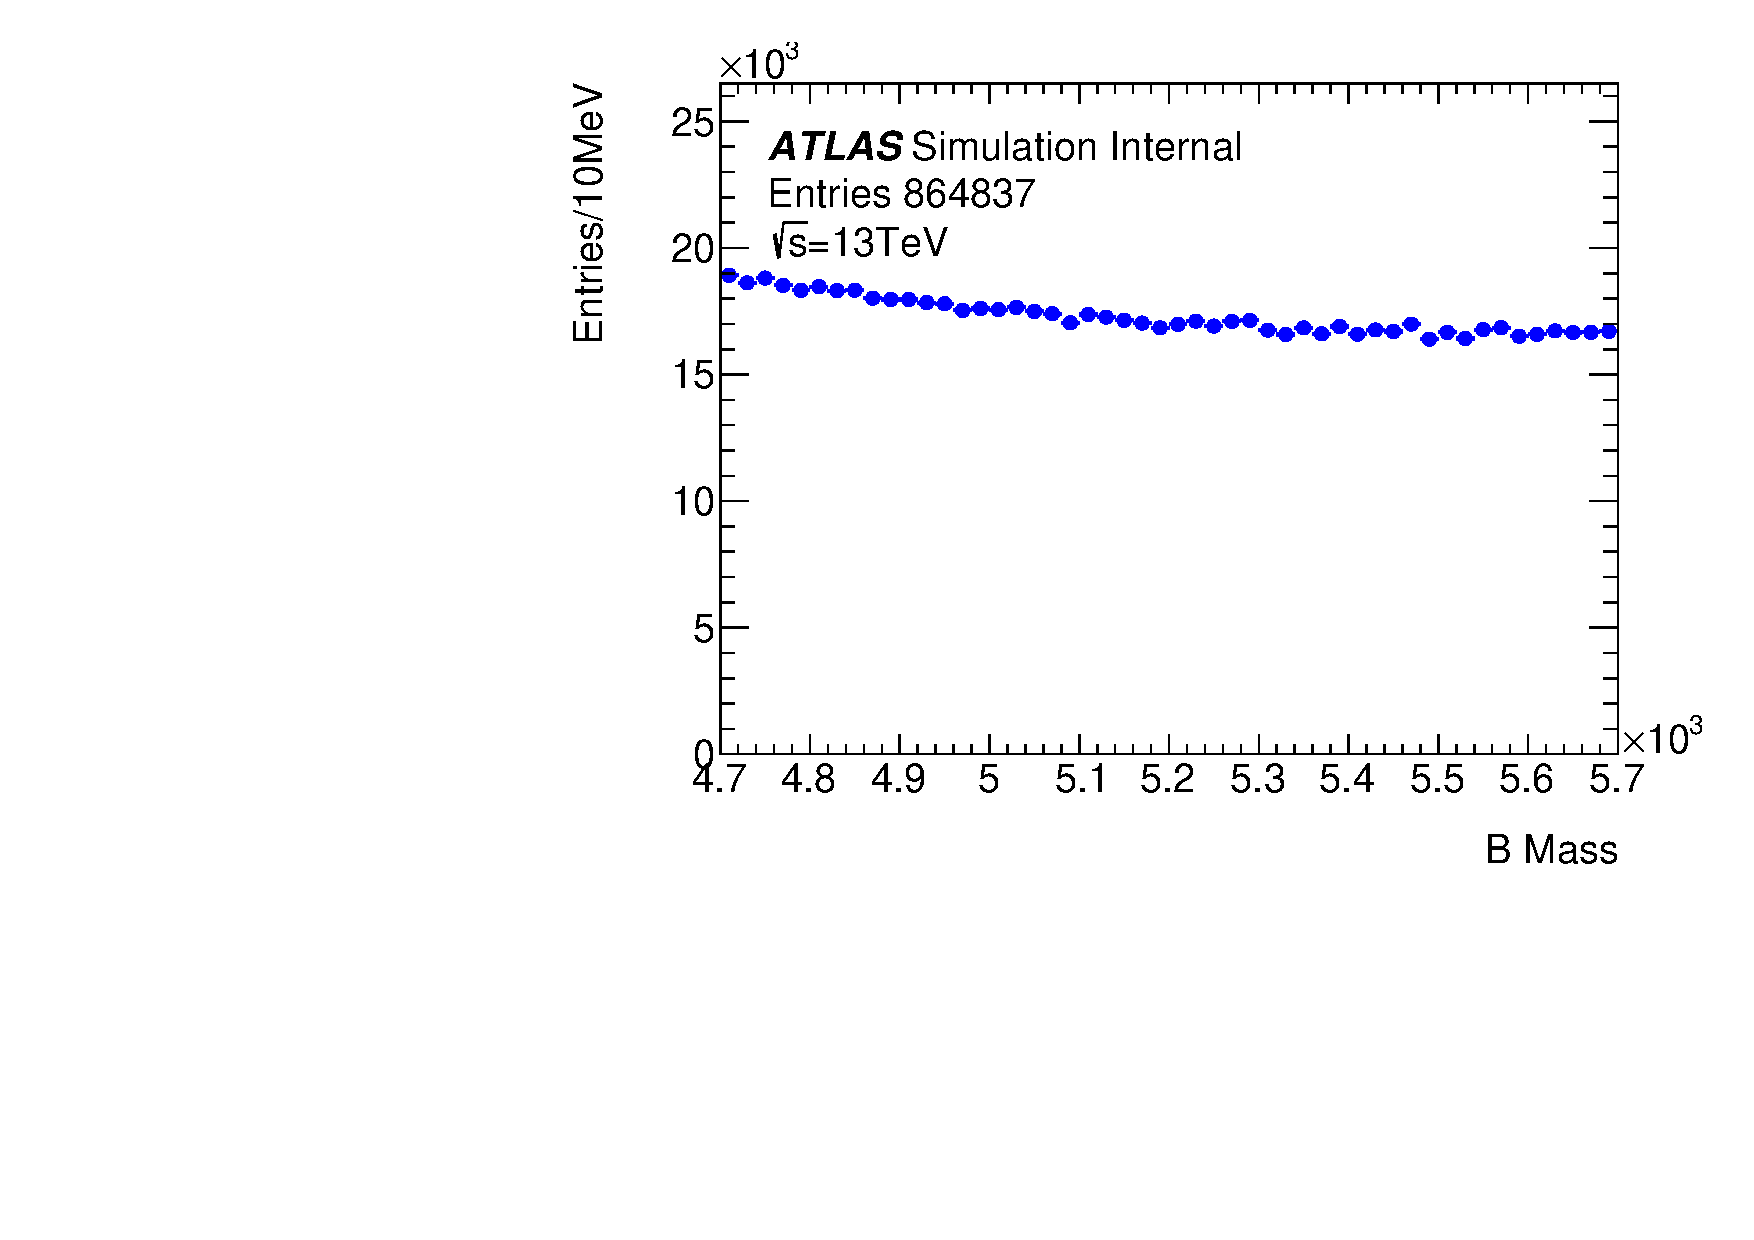
\includegraphics[width=0.45\textwidth]{bplus_components/narrow__864837__unmatched.pdf}
    }
    \caption{\scriptsize The figures show the mass distributions of $B$ candidates classified as
    \textit{combinatorial} and \textit{unmached}. Both distributions are identical in shape.}
    \label{fig:unmatched_combinatorial}
\end{figure}

\clearpage
